\documentclass[11pt,a4paper]{article}
\usepackage{polski}
\usepackage[utf8]{inputenc}
\usepackage{graphicx}
\usepackage{float}
\usepackage[unicode]{hyperref}
\usepackage{geometry}
\usepackage{pdflscape}
\geometry{lmargin=2cm, top=3cm}
\usepackage{longtable}
\usepackage{tabularx}

\author{Architektura Systemów Komputerowych}
\title{Dokumentacja robota typu line follower}
\date{2013/2014}
\listfiles
\begin{document}

\vspace{3cm}
\maketitle
\vspace{2cm}

\begin{center}
\begin{tabularx}{\linewidth}{rl}
  \hline
  Nazwa robota: & \\
  & Żubroń - seksmaszyna \\
  \hline 
  Członkowie drużyny: & \\
  machanika, programowanie, dokumentacja & Szymon Gramza \\
  mechanika, projektowanie PCB & Przemysław Hoffmann \\
  mechanika, wideo & Maciej Królikowski \\
  mechanika, programowanie, dokumentacja & Damian Michalak \\
  mechanika, programowanie, projektowanie PCB & Maciej Sobkowski \\
  mechanika, wideo & Adam Szczesiak \\
  mechanika, programowanie & Kamil Wygralak \\
  \hline
  Prowadzący: & \\
  & dr inż Rafał Klaus \\
  \hline
\end{tabularx} 
\end{center} %end czlonkowie

\newpage
\tableofcontents
\newpage

\section{Wstęp i opis projektu}
Celem projektu było skonstruowanie robota typu Line Follower i wystartowanie w zawodach RoboDay 2014.
Zadaniem robota typu Line Follower jest pokonanie trasy wyznaczonej przez czarną linię umieszczoną na jasnej powierzchni. Wykorzystując odpowiednie sensory i działając według zaimplementowanego algorytmu, nie mogą one z niej zjechać.
\newline Wymagania dotyczące konstrukcji i specyfiki:
\begin{itemize}
  \item Główny obrys robota musi mieścić się na kartce papieru formatu A4,
  \item waga robota nie jest ograniczona
  \item robot musi poruszać się w sposób autonomiczny. Komunikacja z robotem w czasie przejazdu jest zabroniona,
  \item robot powinien być tak zaprojektowany by można było go uruchomić na znak dany przez sędziego.
\end{itemize}
Wymagania dotyczące trasy:
\begin{itemize}
  \item Trasa składać się będzie z białej powierzchni i czarnej linii o szerokości 19$\pm$ 1 mm,
  \item kąt zakrętu o promieniu 0 to maksymalnie 90 stopni,
  \item minimalna odległość między dwiema równoległymi liniami to 210mm,
  \item minimalna odległość między krawędziami planszy a torem to 210mm.
\end{itemize}
\section{Idea rozwiązania}
Stworzony robot spełnia wszystkie warunki dotyczące robotów typu line-follower.
Autonomiczność robota uzyskano poprzez wgranie programu sterującego na mikrokontroler - Atmega8. 
Do wykrywania trasy wykorzystano czujniki odbiciowe CNY70, które przesyłają sygnał do komparatorów.
Następnie komparatory przetwarzają te sygnały i przekierowują je dalej do mikrokontrolera, który analizuje je bezpośrednio zaimplementowanym algorytmem. 
Mikrokontroler steruje pracą silników za pomocą H-mostka, który dostarcza do nich napięcie 12V. Robot posiada jedno źródło zasilania. 
Logika układu jest zasilana z poziomu regulatora napięcia, który otrzymane na wejściu napięcie 12V zmniejsza, dając na wyjściu 5V. 

\section{Mechanika}
  Głównymi komponentami mechanicznej strony robota są:
  \subsection{Konstrukcja nośna}
  Podstawą konstrukcji nośnej i jednocześnie miejscem montażowym elementów elektronicznych są dwie płytki laminatu jednostronnego o wymiarach odpowiednio: 143x169mm oraz 111x56mm. Większa płytka zwana dalej będzie płytką główną, zaś mniejsza zwana także dalej płytką czujnikową. Płytka czujnikowa została umieszczona z przodu konstrukcji i obniżona względem płytki głównej za pomocą 3 dystanserów (śruby i szpilki M3) o łącznej długości 33mm. Zabieg ten umożliwił umieszczenie czujników odbiciowych w optymalnej odległości od podłoża 2-3mm.
  Ścieżki i miejsce przylutowania elementów płytki głównej zostały ulokowane w środkowej części tak, aby możliwe było wygodne przymocowanie pozostałych podzespołów (baterii, silników itd).
  W wyniku wykonania powyższych czynności otrzymano spójną i sztywną konstrukcję mechaniczną.
  \textsc{Schemat konstrukcji}
  Początkowy projekt zakładał jedną płytkę montażową do której planowano zamocować za pomocą dystanserów płytki z układami logicznymi, jednak odrzucono ten pomysł mając na uwadze zmniejszenie całkowitej wagi robota. Zastosowany schemat konstrukcji pozwolił na łatwy dostęp do elementów, głównie do mikroprocesora, co było przydatne podczas programowania. Ponadto utrzymano transparentność oraz ułatwiono ewentualną wymianę podzespołów w przypadku awarii.
  \subsection{Układ jezdny}
  Układ jezdny składa się z części napędowej i mechanicznej. Część napędową tworzą dwa silniki 12V. Silniki umieszczono w tylnej części robota, mocując je za pomocą aluminiowych kątowników które powstały w wyniku zagięcia w połowie długości pod kątem 90 stopni, prostokątnego wycinka blachy o wymiarach 30x60mm. Po zagęciu wykonano nawiercono otwory montownicze.
  
  Część mechaniczna składa się z dwóch elementów. Pierwszym są plastikowo-gumowe koła o wymiarach 43x28mm, pochodzące z zestawu klocków LEGO. Koła są zamontowane na silnikach za pomocą kleju na ciepło.
  
Drugim elementem układu jezdnego jest zamocowany w przedniej części caster, który został wykonany na tokarce w domowych warunkach w celu zmniejszenia kosztów projektu. Przednie koło zapewnia stabilność oraz poziomuje konstrukcję, zmniejsza tarcie i zwiększa zwrotność robota. Dzięki temu zmniejszono także zużycie energii.

\section{Elektrotechnika}
\subsection{Zasilanie}
Zasilanie układu jest dostarczane z pakietu 8 baterii o napięciu 1,5V połączonych szeregowo co daje napięcie 12V.
 W układzie występują trzy różne napięcia:
  \begin{itemize} 
  \item 12V - napięcie silników
  Podawane na H-mostek bezpośrednio z wyjścia baterii.
  Wykorzystywane jest do zasilania silników poprzez sterownik silników.
  \item 5V - napięcie zasilania logiki
  Jest to napięcie wyjściowe otrzymane z regulatora napięcia LM7805, który z wejściowego napięcia 12V daje na wyjściu 5V.
  Wykorzystywane jest ono do zasilania układów logicznych mikrokontrolera, H-mostka i komparatorów oraz do zasilania diód w transoptorach.
  \item 0-5V - regulowane potencjometrem
  Wejściowym napięciem dla potencjometru jest 5V. Jest ono wykorzystywane do regulowania napięcia progowego, używanego do sterowania czułością transoptorów.
  \end{itemize}
  Nie mierzono dokładnego czasu pracy robota na bateriach jednak szacuje się, że wynosi on około 2h.

Inne: odrzucono wariant dodania histerezy (w celu uniknięcia wielu zmian stanów 0->1 i 1->0 spowodowane podobnym co do wartości napięciom wejściowym komparatora pochodzących z transoptorów oraz potencjometru) z powodu konieczności tworzenia dwustronnej płytki co jest trudne do wykonania.
Rozwiązano problem przegrzewania się stabilizatora prze zamocowanie przy nim radiatora oraz przez użycie rezystorów o większym oporze przy diodach CNY70.

[natężenie, moc, napięcie, czas pracy
bez doładowania, waga, stabilizacja, innych danych dotyczących wykonania, problemów któ-
re rozwiązano, wariantów które odrzucono – dlaczego, ...), 
    
  \textsc{schemat bloku zasilania}

\subsection{Silniki}
(opis konstrukcji, parame-
trów technicznych, ogólnych zasad sterowania, innych danych dotyczących wykonania, pro-
blemów które rozwiązano, wariantów które odrzucono – dlaczego

Robot napędzany jest dwoma silnikami firmy Micro motors o oznaczeniach producenta HL 149.6.10 AS.
  Silniki pracują w trybie ciągłej rotacji (continous rotation), w opisanej konfiguracji umieszczono je w tylnej części konstrukcji. 
  Do sterowania prędkością i kierunkiem obrotów silników stosuje się sygnał PWM. Prędkość można regulować dla obu kierunków.
  Charakterystyka zastosowanych silników:
  \begin{itemize}
    \item prędkość kątowa: 60 obr./min.
    \item moment obrotowy: 3,4 kg/cm
    \item napięcie zasilania: 12V DC
    \item wymiary: 40,5x20x38mm
    \item waga: 45g
  \end{itemize}
 Wybór tych silników był motywowany brakiem konieczności stosowania dodatkowej przekładni gdyż mają wysoki moment obrotowy.
 Dodatkowym czynnikiem była niska cena silników, jednak główną motywacją był wysoki współczynnik jakości do ceny.
 
  \textsc{Schemat konstrukcji}

\section{Elektronika}

\subsection{Czujniki}
(zasada działania, parametry, regulacja czułości, innych danych dotyczących wykonania, problemów które rozwiązano,
wariantów które odrzucono – dlaczego, ...),

Do wykrywania koloru zastosowano czujniki CNY70 – układ diody podczerwonej i fototranzystora w jednej obudowie. 
Czujnik wysyła wiązkę promieniowania poprzez nadajnik podczerwieni, a następnie za pomocą fototranzystora, mierzy natężenie światła odbitego. Wyjściem jest sygnał napięciowy, zależny od natężenia światła padającego na ten detektor. Im więcej światła się odbije i dotrze do fotodetektora tym napięcie na wyjściu będzie miało wyższą wartość. Jako że promieniowanie świetlne lepiej odbija powierzchnia jasna ( a ciemna pochłania), dlatego napięcie będzie wyższe na białym materiale.

Specyfikacja czujników CNY70:
\begin{itemize}
  \item Napięcie zasilania diody: 5 V
  \item Maksymalny prąd diody: 50 mA
  \item Maksymalne napięcie kolektor-emiter: 32 V
  \item Maksymalny prąd kolektora: 50 mA
\end{itemize}

\begin{figure}
  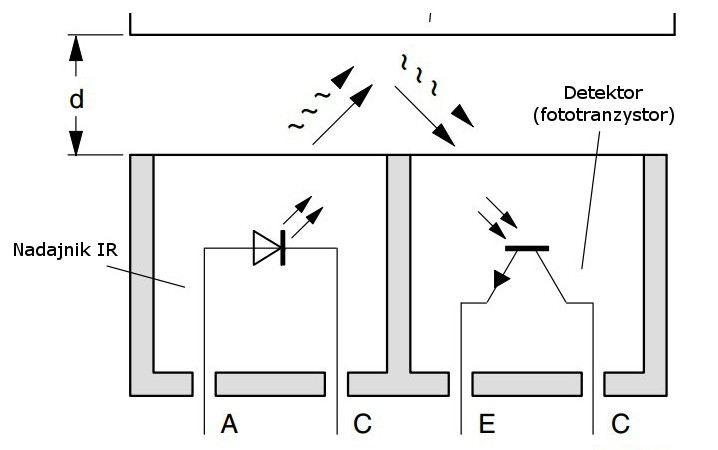
\includegraphics[scale=0.6]{CNY70}
  \caption{Schemat działania transoptora}
\end{figure}

Dokumentacja CNY70 dostępna jest pod adresem: \url{http://botland.com.pl/attachment.php?id_attachment=8}
Do spolaryzowania napięcia na kolektorze fototranzystora wykorzystano rezystory podciągające do VCC o wartości 47k$\Omega$. 
Wyjścia CNY70 dołączone są do pinów PD0-PD6 mikrokontrolera.
Diody podczerwone połączone są szeregowo z rezystorami wartości 330$\Omega$.
Czujniki rozmieszczone są od siebie w odległości 20mm co jest podyktowane standardową szerokością taśmy izolacyjnej (19mm), którą powszechnie stosuje się do wyznaczenia trasy.
Odrzucono koncepcję zastosowania diód sygnalizujących stan czujników w celu oproszczenie schemat płytki.
\textsc{schemat płytki z czujnikami}

\subsection{Sterowanie silnikami} 
Do sterowania pracą silników wykorzystano mostek H. Jest to układ elektrycznym umożliwiający sterowanie kierunkiem działania silników prądu stałego. System PWM reguluje prędkość działania silników. Odrzucono wariant budowy własnego mostka H z tranzystorów z powodu nadmiernej komplikacji układu na płytce.

(zasada sterowania, użyte układy i ich opis w tym parametrów, innych danych dotyczących
wykonania, problemów które rozwiązano, wariantów które odrzucono – dlaczego, ...)

\subsection{Płytka drukowana} Przygotowany robot składa się z dwóch płytek drukowanych: płytki głównej i płytki czujnikowej. Płytka główna jest jednocześnie fundamentem i główną podstawą całego robota. Płytka czujnikowa jest obniżona względem płytki głównej o ok 3cm, aby zapewnić czunikom odpowiednią odległość od trasy (ok 2 mm). Obydwie płytki są ze sobą połączone przewodem 7-pinowym (jeden na każdą czujkę). Odrzucono wariant w którym cała elektronika znajdowałaby się na jednej płytce. Powodem był rozmiar silników jakie udało się nam uzyskać. Silniki mają średnicę ok 3cm, cała płytka główna jest na wysokości ok 6cm od podłoża. Aby zapewnić poprawne działanie czujek, muszą one znajdować się na wysokości ok 2mm od podłoża. Sytuacja ta wymusiła przygotowanie drugiej płytki. Proces przygotowania płytki przebiegał następująco:
\begin {itemize}
    \item przygotowanie schematu płytki w programie EAGLE
    \item wydrukowanie schematu płytki na papierze kredowym
    \item dokładne wyczyszczenie płytki po stronie pokrytej miedzią
    \item ścieranie papierem ściernym niewielkiej ilości miedzi z płytk
    \item podgrzanie płytki na żelazku przez ok 30 sekund
    \item przyprasowanie wydrukowanego schematu płytki, pod wpływem temperatury toner ze schematu przykleja się do miedzi
    \item zanurzenie płytki w wodzie w celu odklejenia kartki ze schematem
    \item zanurzenie płytki w wodzie z wytrawiaczem na ok 15 minut, w celu wytrawienia miedzi w miejscach na których nie ma tonera
    \item wytarcie pozostałego tonera octanem etylu
  \end{itemize}
  Cechy płytki głównej
  \begin{itemize}
    \item schemat przygotowano w programie EAGLE
    \item długość: 171mm
    \item szerokość: 143mm
    \item grubości ścieżek i inne bzdedy PSZEMEK DOKOŃCZ!!!!!!!
    \item dupa dupa chuj
  \end{itemize}



  @@@@@@@@@@@@@@@@@@@@@@ TUTAJ BĘDZIE OBRAZEK PŁYTKI GŁÓWNEJ@@@@@@@@@@@@@@@@

  Cechy płytki czujnikowej
  \begin{itemize}
    \item schemat przygotowano w programie EAGLE
    \item długość: 57mm
    \item szerokość: 111mm
    \item grubości ścieżek i inne bzdedy PSZEMEK DOKOŃCZ!!!!!!!
    \item dupa dupa chuj
  \end{itemize}

  @@@@@@@@@@@@@@@@@@@@@@: TUTAJ BĘDZIE OBRAZEK PŁYTKI CZUJNIKOWEJ@@@@@@@@@@@

Największym problemem podczas przygotowanie płytki było odpowiednie dobranie czasu prasowania płytki z kartką na której był wydrukowany schemat. Po wielu próbach udało się dobrać odpowiedni czas - ok 5 minut. Czas ten zapewnił prawidłowe i całkowite przyklejenie się tonera do miedzi. Niestety podczas wytrawiania napotkano kolejny problem, mianowicie należało wyjąć płytkę z roztworu w odpowiednim czasie. Tak, aby wytrawiła się miedź w miejscach na których nie ma tonera. Jednocześnie nie można trzymać płytki w roztworze za długo, gdyż zacznie się wytrawiać również część miedzi pod tonerem. W obawie przed wytrawieniem się zbyt dużej ilości miedzi, wyjęto płytkę odrobinę za szybko. Później, podczas sprawdzania okazało się, że osobne ścieżki zwierają się ze sobą w kilku miejscach. Problem ten rozwiązano poprzez mechaniczne usunięcie miedzi śrubotkętem.

 i schematy ideowe i montażowe - zasady rozmieszczenia elementów, szeroko-
ści ścieżek (masa, zasilanie, ...), trasowanie i trawienie płytki, narzędzia IT wspomagające, in-
nych danych dotyczących wykonania, problemów które rozwiązano, wariantów które odrzu-
cono – dlaczego, ...).

\section{Mikrokontroler}
(dobór – kryteria, analiza narzędzi uruchomieniowych,...), (opis
wybranego mikrokontrolera, otoczenie mikrokontrolera, innych danych dotyczących wyko-
nania, problemów które rozwiązano, wariantów które odrzucono – dlaczego, ...).
  Robotem steruje mikrokontroler ATmega8.
  Mikrokontroler taktowany jest zewnętrznym oscylatorem kwarcowym o wartości 16MHz. Do pinów PD0-PD4 podpiętych jest 5 niebieskich diod 3mm szeregowo z rezystorami 670$\Omega$ obrazujących stan czujników koloru.
   
  \textsc{schemat mikrokontrolera}

\section{Oprogramowanie}
  \subsection{Algorytm}
  Algorytm sterujący robotem został napisany w języku C. Następnie kod algorytmu został skompilowany w AVR-GCC. Kompilator ten wydany przez firmę ATMEL. Skompilowany program wgrano na mikrokontroler używając programu AVRDUDE. Mikrokontroler jest połączony z wejściem USB komputera za pomocą programatora USB-ASP. 
  Bazą algorytmu jest sterownik PID (człon proporcjonalno całkująco różniczkujący). Dodatkowymi usprawnieniami jest zawracanie po zgubieniu trasy. Program opierra się na głównej pętli w której w pierwszym kroku ssprawdzany jest stan czujników i jeśli wykrywają one linię, to uruchamiany jest algorytm PID, w przeciwnym razie uruchamiana jest procedura odpowiedzialna za powrót na trasę, Odbywa się to poprzez zapamiętanie stanu czujników z poprzedniego odczytu, co dostarcza informacji o prawidłowym kierunku powrotu.

  \subsection{Kod źródłowy}
//z komentarzami, każda linijka numerowana
  Program został zaimplementowany w języku C. Piny PB1-PB2 (sygnał PWM dla serwomechanizmów) oraz PD0-PD4 (diody sygnalizujące stan czujników) zostały ustawione jako wyjściowe, natomiast piny PC1-PC5 (ADC1-ADC5, odczyt stanu czujników) oraz pin PB0 (przycisk uruchamiający) jako piny wejściowe. Odczyt czujników koloru polega na odczycie stanów na pinach PC1-PC5 mikrokontrolera.
  \subsection{Inicjalizacja} (procedury uruchomieniowe, narzędzia i metody, innych danych doty-
czących wykonania, problemów które rozwiązano, wariantów które odrzucono – dlaczego,
...).
  \subsection{Sterowanie}
  Jako algorytm sterowania robotem wykorzystano algorytm regulatora PID.
  \subsection{Pomiar}  
  
\section{Serwisowania i konserwacja} (punkty pomiarowe na płytce i w konstrukcji, analiza
FTA awarii i ich skutków, metody ich usunięcia, innych danych dotyczących wykonania, pro-
blemów które rozwiązano, wariantów które odrzucono – dlaczego, ...).  

\section{Inżynieria oprogramowania i metodyki prowadzenia projektu}
  \subsection{Analiza SWOT członków zespołu}
  
\newgeometry{rmargin=1cm}
\newgeometry{lmargin=1cm}
\newgeometry{top=1cm}
%\footnotesize
\vspace{3cm}
\subsection{Kosztorys}
%\begin{longtable}{|l|r|r@{.}l|r@{.}l|}
\begin{longtable}{|l|r|r|r|}
  \hline
  Element & Ilość & [PLN]/szt & Suma \\
  \hline \hline
  SILNIK & 2 & 5,00 & 10,99\\
  LISTWA ASS02029Z & 1 & 3,00 & 3,00 \\
  LISTWA KOŁK. 1x40pin PROSTA r=2,54mm & 1 & 0,70 & 0,70 \\
  PINHEADER-GNIAZDO 40p PROSTY r=2,54mm & 1 & 1,21 & 1,21 \\
  KOND. CERAMICZNY 22pF & 10 & 0,08 & 0,80 \\
  GNIAZDO BH-10S 10pin PROSTE & 50 & 0,01 & 0,50 \\
  REZ. WĘGL. 0,25W -1K 5\% & 0,1 & 5,01 & 0,50 \\
  LED 3mm ZIELONA-DYFUZYJNA 50 mcd & 0,01 & 15,01 & 0,15 \\
  STAB. 7805 5V/1.5A T0220 & 1 & 1,21 & 1,21 \\
  GNIAZDO DC 5,5/2,1 KĄT. W DRUK-2020 & 1 & 1,00 & 1,00 \\
  ZŁĄCZE AK500/2 r=5mm TAJWAN-NIEB. & 1 & 0,70 & 0,70 \\
  JUMPER r=2,54mm ZAMKNĘTY h=6mm & 0,04 & 5,01 & 0,20 \\
  DŁAWIK 10$\mu$H 160mA 2,5R OSIOWY & 0,10 & 30,00 & 0,30 \\
  DIODA PROST. 1N4007 1A/1000V & 10 & 0,01 & 0,10 \\
  LAMINAT JEDNOSTR. 12x21,5mm GR=1,5m & 1 & 5,81 & 5,81 \\
  TRANSOPTOR & 4 & 2,80 & 11,20 \\
  ATMEGA8A-PU 8kb-FL 1kb-RAM 512b & 1 & 7,50 & 7,50 \\
  NADSIARCZAN SODU-B327 100g & 1 & 4,50 & 4,50 \\
  WIERTŁO 0.8mm & 5 & 1,80 & 9,00 \\
  WIERTŁO 1.0mm & 2 & 1,00 & 1,00 \\
  WIERTŁO 1.2mm SARIUS & 3 & 1,00 & 3,00 \\
  KOND. EL. 4,7$\mu$F/25V 85 C & 10 & 0,05 & 0,50 \\ 
  KOND. KEX47$\mu$F/25V 105 C & 20 & 0,05 & 1,00 \\
  KOND. EL. 10$\mu$F/25V 5x11mm 105 C & 15 & 0,05 & 0,75 \\
  KOND. EL. 100$\mu$F/25V 5x11mm 105 C & 30 & 0,05 & 1,50 \\   
  KOND. EL. 100$\mu$F/50V 8x12mm 105 C & 40 & 0,10 & 0,40 \\ 
  KOND. EL. 470$\mu$F/50V 13x25mm & 1 & 0,60 & 0,60 \\ 
  REZ. WĘGL. 0,25W -75R 5\% & 0,1 & 5,00 & 0,50 \\
  REZ. WĘGL. 0,25W -330R 5\% & 0,1 & 5,00 & 0,50 \\
  REZ. WĘGL. 0,25W -470R 5\% & 0,1 & 5,00 & 0,50 \\
  REZ. WĘGL. 0,25W -1K 5\% & 0,1 & 5,00 & 0,50 \\
  REZ. WĘGL. 0,25W -2,2K 5\% & 0,1 & 5,00 & 0,50 \\
  REZ. WĘGL. 0,25W -1K 5\% & 0,1 & 5,00 & 0,50 \\
  REZ. WĘGL. 0,25W -47K 5\% & 0,1 & 5,00 & 0,50 \\
  MIKRO/SW 6x6mm h=1,5 & 0,1 & 30,0 & 3,00 \\
  STAB. 7805 5V/1,5A T0220 & 2 & 1,20 & 2,40 \\
  KOND. CERAM. 100N/50V/105 r=2,54mm & 0,50 & 10,00 & 0,50 \\
  DŁAWIK 10$\mu$h 160mA 2,5R OSIOWY & 0,02 & 30,00 & 0,60 \\
  LAMINAT JEDNOSTR.19x31 1mm EPOXYD & 1 & 9,00 & 9,00 \\
  SŁUPEK DYST.M3x20mm GWINT Z/W-NIKL. & 4 & 0,75 & 3,00 \\
  NAKRĘTKA M3 -CYNOWANA & 0,04 & 7,00 & 0,28 \\
  ŚRUBA M3 GRZYBEK 10mm & 0,40 & 30,00 & 1,20 \\
  LM 339N DIP14 & 4 & 0,80 & 3,20 \\
  L298N POWER DRIVER SQL15 & 1 & 11,00 & 11,00 \\
  RURA TERM. RT 2,4/1,2 & 1 & 0,80 & 0,80 \\
  L293DNE & 1 & 6,00 & 6,00 \\
  TULEJKA DYST. DR3 6/25mm PLASTIK & 0,02 & 20,00 & 0,40 \\
  POTENCJ. OBROT. B10K LINIOWY L=15mm & 1 & 3,00 & 3,00 \\
  BATERIA 1,5V & 8 & 1,50 & 12,00 \\
  WYTRAWIACZ & 1 & 4,99 & 4,99 \\
  KOSZYCZKI NA BATERIE & 2 & 2,00 & 4,00 \\      
  CZUJNIKI CNY70 & 5 & 2,80 & 14,00 \\ 
  CZUJNIKI CNY70 & 3 & 4,80 & 14,40 \\ 
   &  &  &  \\        
  \hline
\end{longtable}
\restoregeometry

\subsection{Czas pracy} – realny wraz z podziałem zadań i współbieżnością z wyko-
rzystaniem np. wykresów Gantta, problemy z podziałem zadań, problemy z pracą zespołową i
zarządzania czasem – jakie, ich analiza i kreatywne rozwiązania, innych danych dotyczących
wykonania, problemów które rozwiązano, wariantów które odrzucono – dlaczego, analizy
kreatywnej prowadzonego cyklu szkolenia (pomysłu na poprawę ewentualnych wad szkole-
nia )). Inne elementy narzucone prze prowadzących badania studentów V roku.

\subsection{Narzędzie i elementy}
Opis narzędzi i elementów użytych przy realizacji projektu.
\subsection{Narzędzia}
Lista narzędzi:
\begin{itemize}
  \item stacja lutownicza
  \item multiszlifierka precyzyjna z zestawem wymiennych końcówek
  \item zestaw śrubokrętów precyzyjnych
  \item zestaw cążków i kombinerek precyzyjnych
  \item latarka czołowa
  \item pistolet do kleju na ciepło
  \item miernik uniwersalny
  \item ładowarka do akumulatorków
  \item płytka prototypowa
\end{itemize}

Wyżej wymienione narzędzia umożliwiły zamocowanie, unieruchomienie podzespołów na płytkach pcb oraz stworzenie zwartej konstrukcji robota. Ponadto umożliwiły m.in. wiercenie, szlifowanie, matowienie powierzchni, przygotowanie elementów konstrukcyjnych własnej roboty takich jak dystanser przedniego koła w celu wypoziomowania konstrukcji.
Przednie koło zwane dalej casterem zostało 

\section{Uwagi końcowe}

 (powtórzenie najistotniejszych wniosków i uwag ze wskazaniem kie-
runków poprawy konstrukcji robota).

\section{Spisy}
\subsection{Spis rysunków i tabel} 
\subsection{Spis zawartości DVD} (DTR w doc, katalogi elementów elektroniki,
elektrotechniki, mikrokontrolera, zdjęcia dokumentalne, prezentacja PowerPoint – szkole-
niowa dla szkół średnich, wideoklip (od 3 do 5 min wg podanych zasad, inne materiały które
grupa uzna za ważne dla rozwoju i poprawy warszatatów), niezbędne kodeki do wideoklipu .
!!! DTR ma być oddana w okładce plastikowej do której wpina się dziurkowane kartki. Pierw-
sza strona okładki ma być przezroczysta tak aby bez jakiejkolwiek pracy można było odczytać
czego teczka dotyczy (widoczna pierwsza strona DTR). Na końcu zamocowany w kopercie pa-
pierowej DVD (podpisany). 

\section{Literatura}
Literatura pomocna przy tworzeniu robota.

\end{document}
